\section{Auswertung} % (fold)
\label{sec:auswertung}

Alle Fehlerrechnungen wurden mithilfe Gaußscher Fehlerfortpflanzung errechnet.

\begin{equation}
	\Delta f(x_\text{1}\text{,...,}x_\text{n}) = \sqrt{\sum_\text{i=0}^\text{n} \left(\frac{\partial f}{\partial x_\text{i}} \Delta x_\text{i}\right)^2}
\end{equation}

Dafür ist die Python Bibliothek \textit{uncertainties} benutzt worden.

\subsection{Untersuchung eines Reflexklystrons} % (fold)
\label{sub:untersuchung_der_}

\begin{figure}
	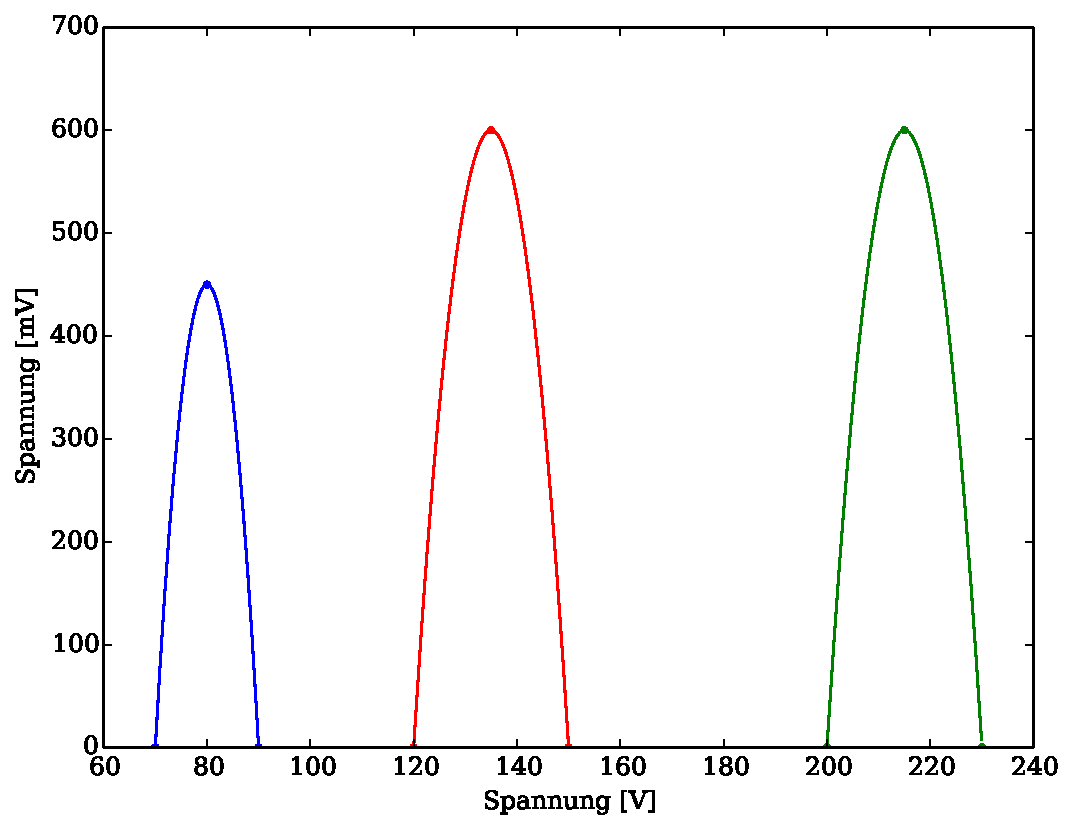
\includegraphics[width = 14cm]{pic/ModenDiagramm.pdf}
	\caption[]{Modus-Diagramm des Reflexklystrons bei einer Abstimmung auf $\SI{9}{\giga\hertz}$. Die Leistung der Amplitude ist proportional zur Spannung.}
	\label{mode}
\end{figure}

Nach der Abstimmung des Klystrons auf $\SI{9}{\giga\hertz}$ und der Bestimmung der Modenbreiten und Amplituden, hat sich das in Abbildung \ref{mode} dargestellte Modus-Diagramm ergeben.
Für die elektronische Bandbreite $B$ des Klystrons hat sich 

\begin{eqnarray}
	B &=& \frac{f'-f''}{V'-V''}\\
	\Rightarrow B &=& \SI{2.1(7)}{\hertz\per\volt}
\end{eqnarray}

ergeben.

Die benutzten Dateien sind in Tabelle \ref{v1} aufgelistet.

\begin{table}
\centering
\begin{tabular}{r r r r r r}
	Mode & $V_\text{0}[\SI{}{\volt}]$ & $V_\text{1}[\SI{}{\volt}]$ & $V_\text{2}[\SI{}{\volt}]$ & $A_\text{0}[\SI{}{\milli\volt}]$ & $f[\SI{}{\mega\hertz}]$ \\
	\hline
	\hline
	1 & 215 & 200 & 230 & 600 & 9000.5\\
	2 & 185 & 120 & 150 & 600 & 9005.0\\
	3 &  80 &  70 &  90 & 450 & 9010.5\\
	\hline
\end{tabular}
\caption{Messwerte zur Darstellung des Modus-Diagramms.}
\begin{tabular}{r r r r r r}
	$V_\text{0}[\SI{}{\volt}]$ & $V'[\SI{}{\volt}]$ & $V''[\SI{}{\volt}]$ & $f_\text{0}[\SI{}{\mega\hertz}]$  & $f'[\SI{}{\mega\hertz}]$ & $f''[\SI{}{\mega\hertz}]$ \\
	\hline
	\hline
	215 & 225 & 205 & 9001.0 & 9024.0 & 8982.5\\
	\hline
\end{tabular}
\caption{Messwerte zur Bestimmung der Banbreite $B$ des Klystrons.}
\label{v1}
\end{table}

